%----------------------------------------------------------------------------------------
%	PACKAGES AND THEMES
%----------------------------------------------------------------------------------------
\documentclass[aspectratio=169,xcolor=dvipsnames]{beamer}
\usetheme{Simple}
\usepackage{setspace} % Incluye esto en el preámbulo
\documentclass{beamer}
\setbeamertemplate{caption}[numbered] % Habilita numeración de tablas
\usepackage{hyperref}
\usepackage{graphicx} % Allows including images
\usepackage{booktabs} % Allows the use of \toprule, \midrule and \bottomrule in tables
\usepackage{tikz}
\usetikzlibrary{shapes.geometric, arrows, positioning, calc} % Incluye calc
\tikzstyle{startstop} = [ellipse, minimum width=2.5cm, minimum height=1cm, text centered, draw=black, fill=red!30]
\tikzstyle{process} = [rectangle, rounded corners, minimum width=2.5cm, minimum height=1cm, text centered, draw=black, fill=blue!30]
\tikzstyle{arrow} = [thick,->,>=stealth]

%----------------------------------------------------------------------------------------
%	TITLE PAGE
%----------------------------------------------------------------------------------------

% The title
\title[short title]{Clusterización de Nubes Potencialmente Precipitables en Cusco durante el periodo 12/2023 al 04/2024}
\subtitle{Proyecto de Investigación}

\author[Pin-Yen] {Araujo R., Robert$^{1}$, Rivera F., Alexis$^{2}$ y Salinas J., Allen$^{3}$.}
\institute[Universidad Nacional Agraria La Molina] % Your institution may be shorthand to save space
{
    % Your institution for the title page
    Departamento de Física y Meteorología\\
    Universidad Nacional Agraria La Molina\\
    Curso: Técnicas de Programación II\\
    Docente: MSc. Príncipe A, Erick. romelprincipea@gmail.com
    \vskip 3pt
}
\date{Diciembre 20, 2024} % Date, can be changed to a custom date
%----------------------------------------------
%	PRESENTATION SLIDES
%----------------------------------------------
\begin{document}

\begin{frame}
    % Print the title page as the first slide
    \titlepage
\end{frame}

\begin{frame}{Contenido}
    % Throughout your presentation, if you choose to use \section{} and \subsection{} commands, these will automatically be printed on this slide as an overview of your presentation
    \tableofcontents
\end{frame}
%------------------------------------------------
\section{Introducción}
\begin{frame}{Introducción} 
    La identificación y análisis de patrones climáticos mediante datos satelitales es esencial para comprender fenómenos meteorológicos complejos~\cite{b1}.
    % Inserción de la imagen 
    \begin{figure}
    \centering
    \includegraphics[width=0.45\textwidth]{intro/000479355W.jpg} % Cambia la ruta por la ubicación de tu imagen
    \caption{Lluvia en la región de Cusco}
    \vspace{-7pt}
    % Fuente debajo de la imagen con tamaño reducido
    {\tiny
        \setlength{\baselineskip}{-1pt}
        \textbf{Fuente:} Andina. (2018)
    }
    \end{figure}
\end{frame}
\begin{frame}{Introducción}
        Se utilizó datos de temperatura de brillo de la banda 13 del GOES-16, apoyado del algoritmo de clustering K-means para identificar de nubes potencialmente precipitables. 

    % Inserción de la imagen 
    \begin{figure}
    \centering
    \includegraphics[width=0.5\textwidth]{intro/14213141670_1d34813e99_o.png} % Cambia la ruta por la ubicación de tu imagen
    \caption{Satelite GOES}
    \vspace{-7pt}
    % Fuente debajo de la imagen con tamaño reducido
    {\tiny
        \setlength{\baselineskip}{1pt}
        \textbf{Fuente:} NOAA Satellites. (2011)
    }
    \end{figure}
\end{frame}
%------------------------------------------------
\section{Antecedentes}
\begin{frame}{Antecedentes}
    \begin{block}{~\cite{b3}}
        En esta investigación se aplicó el algoritmo de agrupamiento no supervisado k-means/k-means++ a imágenes del satélite GOES-13 para la región de Sudamérica, entre 12/2010 y 11/2016. El objetivo fue clasificar nubes según su temperatura de brillo media.
    \end{block}
    
    \begin{block}{~\cite{b4}}
        Se utilizó el algoritmo fuzzy k-means (FKM) para clasificar capas detectadas por el lidar CALIPSO (algoritmo supervisado) como nubes o aerosoles. Las clasificaciones de FKM coincidieron en más del 94\% con las de COCA en la troposfera.
    \end{block}
    
    
\end{frame}
%------------------------------------------------
\section{Objetivos}
\begin{frame}{Objetivos}
    
    \begin{block}{Objetivo General}
        Aplicar técnicas de clusterización a datos satelitales de temperatura de brillo de la banda 13 del GOES-16 para identificar y analizar patrones de nubes potencialmente precipitables sobre el departamento de Cusco durante el periodo 12/2023 al 04/2024.
    \end{block}

    \begin{block}{Objetivos Específicos}
        \begin{itemize}
            \item Determinar el número de K óptimo mediante el método del codo para clusterizar los datos de temperatura de brillo.
            \item Comparar los clusters obtenidos con datos de precipitación de estaciones meteorológicas del SENAMHI dentro del departamento de Cusco.
        \end{itemize}
    \end{block}
\end{frame}

%------------------------------------------------
\section{Marco Teórico}
\begin{frame}{Marco Teórico}
    % Definición o descripción con tamaño reducido
    \begin{block}{\small Banda 13: IR de “Onda larga limpio”} % Título más pequeño
        {\tiny % Se aplica el tamaño pequeño a todo el contenido dentro del bloque
        \begin{itemize}
            \item \textbf{Longitud de onda:} 10,3 μm.
            \item \textbf{Resolución:} 2 km.
            \item \textbf{Disponibilidad:} Todo el día.
            \item \textbf{Principal Aplicación:} Identificación de Nubes.
        \end{itemize}
        }
    \end{block}

    % Inserción de la imagen 
    \begin{figure}
    \centering
    \includegraphics[width=0.3\textwidth]{MarcoTeoric/Ref1.jpg} % Cambia la ruta por la ubicación de tu imagen
    \caption{Imagen de la banda 13 IR para la región de Perú.}
    % Fuente debajo de la imagen con tamaño reducido
    \vspace{-7pt}
    {\tiny
        \textbf{Fuente:} Adaptado de SENAMHI (2024). Satélite GOES-16. 
    }
    \end{figure}
\end{frame}

%------------------------------------------------
\begin{frame}{Nubes Precipitables}
   \begin{table}[h]
    \centering
    \scriptsize % Reduce el tamaño del texto dentro de la tabla
    \resizebox{0.5\textwidth}{!}{ % Reduce el ancho total al 50% de la página
    \begin{tabular}{l l l}
        \toprule
        \textbf{Género} & \textbf{Abreviación} & \textbf{Altura en la atmósfera} \\ 
        \midrule
        Cirrus & Ci & Alta \\
        Cirrocumulus & Cc & Alta \\
        Cirrostratus & Cs & Alta \\
        Altocumulus & Ac & Media \\
        Altostratus & As & Media \\
        Nimbostratus & Ns & Baja \\
        Stratus & St & Baja \\
        Cumulus & Cu & Nubes convectivas \\
        Cumulonimbus & Cb & Nubes convectivas \\
        \bottomrule
    \end{tabular}
    }
    \caption{Género, abreviación y altura en la atmósfera de las nubes.}
    \scriptsize \textbf{Fuente:} Adaptado de la WMO (World Meteorological Organization) e Iribarne J.V. (1980), citado por Romero~\cite{b7}.
    \end{table}
\end{frame}
%------------------------------------------------

\begin{frame}{Clustering}
    \begin{columns}

        \column{0.5\textwidth}
        \begin{figure}
            \centering
            \includegraphics[width=\linewidth]{MarcoTeoric/cluster1.png}
            {\footnotesize % Tamaño reducido
            \caption{Ejemplos de clusters}
            \label{fig6}
            \vspace{-7pt}
            {\tiny
                \textbf{Fuente:} Expósito et. al. (s/f)
            }}
        \end{figure}
        \column{0.5\textwidth}
        \begin{figure}
            \centering
            \includegraphics[width=\linewidth]{MarcoTeoric/cluster2.png}
            {\footnotesize % Tamaño reducido
            \caption{Ejemplos de clusters}
            \label{fig7}
            \vspace{-7pt}
            {\tiny
                \textbf{Fuente:} Expósito et. al. (s/f)
            }}
        \end{figure}

    \end{columns}
\end{frame}

%------------------------------------------------

%------------------------------------------------
\section{Metodología}
\begin{frame}{Metodología}
    \begin{figure}[H]
    \centering
    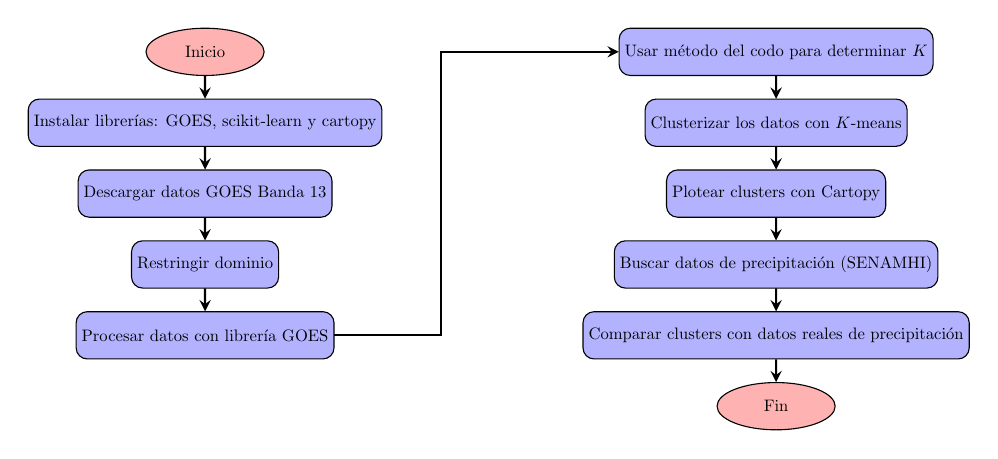
\begin{tikzpicture}[node distance=1.5cm, auto, scale=0.9, every node/.style={scale=0.6}] % Escala ajustada

        % Primera columna
        \node (start) [startstop] {Inicio};
        \node (step1) [process, below of=start] {Instalar librerías: GOES, scikit-learn y cartopy};
        \node (step2) [process, below of=step1] {Descargar datos GOES Banda 13};
        \node (step3) [process, below of=step2] {Restringir dominio};
        \node (step4) [process, below of=step3] {Procesar datos con librería GOES};

        % Segunda columna (alineada con el inicio de la primera columna)
        \node (step5) [process, right=4.5cm of start] {Usar método del codo para determinar $K$};
        \node (step6) [process, below of=step5] {Clusterizar los datos con $K$-means};
        \node (step7) [process, below of=step6] {Plotear clusters con Cartopy};
        \node (step8) [process, below of=step7] {Buscar datos de precipitación (SENAMHI)};
        \node (step9) [process, below of=step8] {Comparar clusters con datos reales de precipitación};
        \node (stop) [startstop, below of=step9] {Fin};

        % Conexiones de la primera columna
        \draw [arrow] (start) -- (step1);
        \draw [arrow] (step1) -- (step2);
        \draw [arrow] (step2) -- (step3);
        \draw [arrow] (step3) -- (step4);

        % Conexión entre columnas
        \draw [arrow] (step4.east) -- ++(1.5,0) |- (step5.west);

        % Conexiones de la segunda columna
        \draw [arrow] (step5) -- (step6);
        \draw [arrow] (step6) -- (step7);
        \draw [arrow] (step7) -- (step8);
        \draw [arrow] (step8) -- (step9);
        \draw [arrow] (step9) -- (stop);

    \end{tikzpicture}
    \caption{Flujograma del proceso metodológico.}
    \label{fig6}
    \end{figure}
\end{frame}

%------------------------------------------------
\begin{frame}{Zona de Estudio}
    La zona de estudio es el departamento Cusco, ubicado en la región andina de Perú.
    \begin{figure}
            \centering
            \includegraphics[width=0.28\linewidth]{codigos/cusco.png}
            {\footnotesize % Tamaño reducido
            \caption{Mapa de Ubicación del departamento Cusco en Perú}
            \label{fig2}
            }
    \end{figure}
\end{frame}

\begin{frame}{Software}
    
    \begin{block}{Lenguaje de Programación}
        Python.
    \end{block}

    \begin{block}{Librerías en Python}
        GOES para instalar y manejar datos GOES, scikit-learn para aplicar el algoritmo K-means y Cartopy para visualización de los resultados.
    \end{block}
\end{frame}

\begin{frame}{Datos de Imágenes GOES}
    
    \begin{itemize}
        \item \textbf{Satélite:} GOES-16.
        \item \textbf{Banda:} 13.
        \item \textbf{Producto:} CMI.
        \item \textbf{Resolución espacial:} 2 km.
        \item \textbf{Periodo:} 12/2023 al 04/2024.
    \end{itemize}
\end{frame}
\begin{frame}{Datos de Imágenes GOES}
    \begin{table}[h]
        \centering
        \resizebox{\textwidth}{!}{ % Ajusta la tabla al ancho de la diapositiva
        \begin{tabular}{l l l l l}
        \toprule
        \textbf{12/2023} & \textbf{01/2024} & \textbf{02/2024} & \textbf{03/2024} & \textbf{03/2024} \\ 
        \midrule
        08/12/2023 (22:30 UTC) & 24/01/2024 (05:30 UTC) & 10/02/2024 (05:30 UTC) & 09/03/2024 (20:30 UTC) & 13/04/2024 (05:30 UTC) \\ 
        29/12/2023 (20:30 UTC) &  & 19/02/2024 (20:30 UTC) & 16/03/2024 (20:30 UTC) & \\ 
         &  &  & 17/03/2024 (09:00 horas UTC) & \\        
        \bottomrule
        \end{tabular}
        }
        \caption{Fecha y hora de los datos GOES para cada mes dentro del periodo 12/2023 al 04/2024} 
        \label{tab2} 
    \end{table}
\end{frame}

\begin{frame}{Algoritmo k-means}
    \begin{columns}

        \column{0.5\textwidth}
        \begin{figure}
            \centering
            \includegraphics[width=1.\linewidth]{MarcoTeoric/codo.PNG}
            {\footnotesize % Tamaño reducido
            \caption{Método del codo}
            \label{fig6}}
        \end{figure}
    \end{columns}
\end{frame}

%------------------------------------------------
\begin{frame}{Estaciones Meteorólogicas en la Región de Cusco}
    \centering
    \begin{table}
        \centering
        \begin{tabular}{l l l l l}
            \toprule
            \textbf{Nombre} & \textbf{Latitud} & \textbf{Longitud} & \textbf{Altura (m)} & \textbf{Tipo} \\
            \midrule
            Quincemil        & 13°13'44.15''S   & 70°45'15.84''W   & 651  & Convencional \\
            Chacllabamba     & 13°6'30.77''S    & 71°43'12.01''W   & 2699 & Convencional \\
            Chontachaca      & 13°1'26''S       & 71°28'4''W       & 872  & Convencional \\
            Colquepata       & 13°21'47.27''S   & 71°40'24.1''W    & 3696 & Convencional \\
            Sibinacocha      & 13°55'19.7''S    & 71°1'5.63''W     & 4880 & Automática \\
            Caicay           & 13°35'59.96''S   & 71°42'1''W       & 3117 & Convencional \\
            Calca            & 13°19'59.97''S   & 71°57'18.85''W   & 2921 & Automática \\
            Urubamba         & 13°18'18.6''S    & 72°7'28.4''W     & 2850 & Convencional \\
            Anta Ancachuro   & 13°28'20.71''S   & 72°13'7.54''W    & 3324 & Convencional \\
            Sicuani          & 14°14'14.5''S    & 71°14'12.1''W    & 3534 & Automática \\
            Aymaña           & 13°52'22.03''S   & 70°40'3.34''W    & 4175 & Automática \\
            Pichari          & 12°31'19.9''S    & 73°50'22.28''W   & 570  & Automática \\
            \bottomrule
        \end{tabular}
        \caption{Estaciones Meteorológicas en la región de estudio}
    \end{table}

\end{frame}



%------------------------------------------------
\begin{frame}{Librerías y Descarga de datos GOES}
    \begin{columns}

        \column{0.5\textwidth}
        \begin{figure}
            \centering
            \includegraphics[width=\linewidth]{codigos/librerias.PNG}
            {\footnotesize % Tamaño reducido
            \caption{Librerias Utilizadas}
            \label{fig4}
            }
        \end{figure}
        \column{0.5\textwidth}
        \begin{figure}
            \centering
            \includegraphics[width=\linewidth]{codigos/descarga.PNG}
            {\footnotesize % Tamaño reducido
            \caption{Código para descarga de datos GOES}
            \label{fig5}
            }
        \end{figure}

    \end{columns}
\end{frame}
%------------------------------------------------
\begin{frame}{Dominio y Tratamiento del Array}
    \begin{columns}

        \column{0.5\textwidth}
        \begin{figure}
            \centering
            \includegraphics[width=\linewidth]{codigos/dominio.PNG}
            {\footnotesize % Tamaño reducido
            \caption{Definición del Dominio (Zona de Estudio)}
            \label{fig6}
            }
        \end{figure}
        \column{0.5\textwidth}
        \begin{figure}
            \centering
            \includegraphics[width=\linewidth]{codigos/tratamiento.PNG}
            {\footnotesize % Tamaño reducido
            \caption{Tratamiento del Array CMI}
            \label{fig7}
            }
        \end{figure}

    \end{columns}
\end{frame}
%------------------------------------------------
\begin{frame}{Método del Codo}
    \begin{columns}
        \column{0.5\textwidth}
        \begin{figure}
            \centering
            \includegraphics[width=0.8\linewidth]{codigos/entreno.PNG}
            {\footnotesize % Tamaño reducido
            \caption{Entrenamiento para el Método del codo}
            \label{fig8}
            }
        \end{figure}
        \begin{figure}
            \centering
            \includegraphics[width=0.70\linewidth]{codigos/codo.PNG}
            {\footnotesize % Tamaño reducido
            \caption{Aplicación del Método del Codo}
            \label{fig9}
            }
        \end{figure}
        \column{0.5\textwidth}
        \begin{figure}
            \centering
            \includegraphics[width=0.90\linewidth]{codigos/codo1.PNG}
            {\footnotesize % Tamaño reducido
            \caption{Resultado}
            \label{fig10}
            }
        \end{figure}

    \end{columns}
\end{frame}
%------------------------------------------------
\begin{frame}{Definición Clusters y Tratamiento de Array}
    \begin{columns}

        \column{0.5\textwidth}
        \begin{figure}
            \centering
            \includegraphics[width=\linewidth]{codigos/definicion.PNG}
            {\footnotesize % Tamaño reducido
            \caption{Definición de la cantidad de Clusters}
            \label{fig11}
            }
        \end{figure}
        \column{0.5\textwidth}
        \begin{figure}
            \centering
            \includegraphics[width=\linewidth]{codigos/tratamiento2.PNG}
            {\footnotesize % Tamaño reducido
            \caption{Tratamiento del Array por segunda vez}
            \label{fig12}
            }
        \end{figure}

    \end{columns}
\end{frame}
%------------------------------------------------
\begin{frame}{Resultado Preliminar y Arreglos (Mapa Final)}
    \begin{columns}

        \column{0.5\textwidth}
        \begin{figure}
            \centering
            \includegraphics[width=0.75\linewidth]{codigos/resultadopre.PNG}
            {\footnotesize % Tamaño reducido
            \caption{Resultado Preliminar con Imshow}
            \label{fig13}
            }
        \end{figure}
        \column{0.5\textwidth}
        \begin{figure}
            \centering
            \includegraphics[width=\linewidth]{codigos/arreglos.PNG}
            {\footnotesize % Tamaño reducido
            \caption{Arreglos para los Mapas Finales}
            \label{fig14}
            }
        \end{figure}

    \end{columns}
\end{frame}
%------------------------------------------------
\begin{frame}{Ploteo con Temperatura de Brillo}
    \begin{figure}
        \centering
        \includegraphics[width=0.80\linewidth]{codigos/plottemp.PNG}
        {\footnotesize % Tamaño reducido
        \caption{Ploteo con la Temperatura de Brillo}
        \label{fig15}
        }
    \end{figure}
\end{frame}
%------------------------------------------------
\begin{frame}{Ploteo con Clusters}
    \begin{figure}
        \centering
        \includegraphics[width=0.80\linewidth]{codigos/plotclus.PNG}
        {\footnotesize % Tamaño reducido
        \caption{Ploteo con los Clusters}
        \label{fig16}
        }
    \end{figure}
\end{frame}
%------------------------------------------------
\section{Resultados y Discusiones}
\begin{frame}{Resultados y Discusiones (08/12/2023 a las 22:30 horas UTC)}
\begin{figure}
    \centering
    \includegraphics[width=0.4\linewidth]{Resultados/resultado1a.png}
    \caption{Mapa de temperatura de brillo para el 08/12/2023 a las 22:30 horas UTC}
    \label{fig6}
\end{figure}
\end{frame}
%------------------------------------------------
\begin{frame}{Resultados y Discusiones (08/12/2023 a las 22:30 horas UTC)}
    \begin{columns}

        % Primera columna: Mapa de clusters
        \column{0.75\textwidth} % Ajusta el ancho de la columna
        \begin{figure}
            \centering
            \includegraphics[width=0.6\linewidth]{Resultados/resultado1b.png}
            {\footnotesize % Tamaño reducido
            \caption{Mapa de clusters para el 08/12/2023 a las 22:30 horas UTC.}
            \label{fig7}
            }
        \end{figure}

        % Segunda columna: Tabla con valores de los clusters
        \column{0.25\textwidth} % Ajusta el ancho de la columna
        \centering
        \begin{table}[h!]
            \centering
            {\footnotesize % Tamaño reducido para la tabla
            \begin{tabular}{|c|c|}
                \hline
                \textbf{Cluster} & \textbf{Valor} \\
                \hline
                Cluster 0 & 230.76 \\
                Cluster 1 & 281.75 \\
                Cluster 2 & 256.87 \\
                Cluster 3 & 258.65 \\                
                \hline
            \end{tabular}
            \caption{Media de cada cluster para el 08/12/2023 a las 22:30 horas UTC.}
            }
        \end{table}

    \end{columns}
\end{frame}
%------------------------------------------------
\begin{frame}{Resultados y Discusiones (29/12/2023 a las 20:30 horas UTC)}
\begin{figure}
    \centering
    \includegraphics[width=0.4\linewidth]{Resultados/resultado2a.png}
    \caption{Mapa de temperatura de brillo para el 29/12/2023 a las 20:30 horas UTC}
    \label{fig8}
\end{figure}
\end{frame}
%------------------------------------------------
\begin{frame}{Resultados y Discusiones (29/12/2023 a las 20:30 horas UTC)}
    \begin{columns}

        % Primera columna: Mapa de clusters (más grande)
        \column{0.75\textwidth} % Ajusta el ancho de la columna
        \begin{figure}
            \centering
            \includegraphics[width=0.60\linewidth]{Resultados/resultado2b.png}
            {\footnotesize % Tamaño reducido
            \caption{Mapa de clusters para el 29/12/2023 a las 22:30 horas UTC.}
            \label{fig9}
            }
        \end{figure}

        % Segunda columna: Tabla con valores de los clusters
        \column{0.25\textwidth} % Ajusta el ancho de la columna
        \centering
        \begin{table}[h!]
            \centering
            {\footnotesize % Tamaño reducido para la tabla
            \begin{tabular}{|c|c|}
                \hline
                \textbf{Cluster} & \textbf{Valor} \\
                \hline
                Cluster 0 & 236.89 \\
                Cluster 1 & 286.79 \\
                Cluster 2 & 261.33 \\
                Cluster 3 & 218.00 \\                
                \hline
            \end{tabular}
            \caption{Media de cada cluster para el 29/12/2023 a las 22:30 horas UTC.}
            }
        \end{table}

    \end{columns}
\end{frame}
%------------------------------------------------
\begin{frame}{Resultados y Discusiones (24/01/2024 a las 05:30 horas UTC)}
\begin{figure}
    \centering
    \includegraphics[width=0.4\linewidth]{Resultados/resultado3a.png}
    \caption{Mapa de temperatura de brillo para el 24/01/2024 a las 05:30 horas UTC}
    \label{fig10}
\end{figure}
\end{frame}
%------------------------------------------------
\begin{frame}{Resultados y Discusiones (24/01/2024 a las 05:30 horas UTC)}
    \begin{columns}

        % Primera columna: Mapa de clusters (más grande)
        \column{0.75\textwidth} % Ajusta el ancho de la columna
        \begin{figure}
            \centering
            \includegraphics[width=0.60\linewidth]{Resultados/resultado3b.png}
            {\footnotesize % Tamaño reducido
            \caption{Mapa de clusters para el 24/01/2024 a las 05:30 horas UTC.}
            \label{fig11}
            }
        \end{figure}

        % Segunda columna: Tabla con valores de los clusters
        \column{0.25\textwidth} % Ajusta el ancho de la columna
        \centering
        \begin{table}[h!]
            \centering
            {\footnotesize % Tamaño reducido para la tabla
            \begin{tabular}{|c|c|}
                \hline
                \textbf{Cluster} & \textbf{Valor} \\
                \hline
                Cluster 0 & 239.48 \\
                Cluster 1 & 283.10 \\
                Cluster 2 & 262.60 \\
                Cluster 3 & 220.71 \\                
                \hline
            \end{tabular}
            \caption{Media de cada cluster para el 24/01/2024 a las 05:30 horas UTC.}
            }
        \end{table}

    \end{columns}
\end{frame}
%------------------------------------------------
\begin{frame}{Resultados y Discusiones (10/02/2024 a las 05:30 horas UTC)}
\begin{figure}
    \centering
    \includegraphics[width=0.4\linewidth]{Resultados/resultado8a.png}
    \caption{Mapa de temperatura de brillo para el 10/02/2024 a las 05:30 horas UTC}
    \label{fig12}
\end{figure}
\end{frame}
%------------------------------------------------
\begin{frame}{Resultados y Discusiones (10/02/2024 a las 05:30 horas UTC)}
    \begin{columns}

        % Primera columna: Mapa de clusters (más grande)
        \column{0.75\textwidth} % Ajusta el ancho de la columna
        \begin{figure}
            \centering
            \includegraphics[width=0.60\linewidth]{Resultados/resultado8b.png}
            {\footnotesize % Tamaño reducido
            \caption{Mapa de clusters para el 10/02/2024 a las 05:30 horas UTC.}
            \label{fig13}
            }
        \end{figure}

        % Segunda columna: Tabla con valores de los clusters
        \column{0.25\textwidth} % Ajusta el ancho de la columna
        \centering
        \begin{table}[h!]
            \centering
            {\footnotesize % Tamaño reducido para la tabla
            \begin{tabular}{|c|c|}
                \hline
                \textbf{Cluster} & \textbf{Valor} \\
                \hline
                Cluster 0 & 211.34 \\
                Cluster 1 & 285.10 \\
                Cluster 2 & 235.53 \\
                Cluster 3 & 267.62 \\                
                \hline
            \end{tabular}
            \caption{Media de cada cluster para el 10/02/2024 a las 05:30 horas UTC.}
            }
        \end{table}

    \end{columns}
\end{frame}
%------------------------------------------------
\begin{frame}{Resultados y Discusiones (19/02/2024 a las 20:30 horas UTC)}
\begin{figure}
    \centering
    \includegraphics[width=0.4\linewidth]{Resultados/resultado4a.png}
    \caption{Mapa de temperatura de brillo para el 19/02/2024 a las 20:30 horas UTC}
    \label{fig14}
\end{figure}
\end{frame}
%------------------------------------------------
\begin{frame}{Resultados y Discusiones (19/02/2024 a las 20:30 horas UTC)}
    \begin{columns}

        % Primera columna: Mapa de clusters (más grande)
        \column{0.75\textwidth} % Ajusta el ancho de la columna
        \begin{figure}
            \centering
            \includegraphics[width=0.60\linewidth]{Resultados/resultado4b.png}
            {\footnotesize % Tamaño reducido
            \caption{Mapa de clusters para el 19/02/2024 a las 20:30 horas UTC}
            \label{fig15}
            }
        \end{figure}

        % Segunda columna: Tabla con valores de los clusters
        \column{0.25\textwidth} % Ajusta el ancho de la columna
        \centering
        \begin{table}[h!]
            \centering
            {\footnotesize % Tamaño reducido para la tabla
            \begin{tabular}{|c|c|}
                \hline
                \textbf{Cluster} & \textbf{Valor} \\
                \hline
                Cluster 0 & 238.71 \\
                Cluster 1 & 288.73 \\
                Cluster 2 & 218.07 \\
                Cluster 3 & 263.29 \\                
                \hline
            \end{tabular}
            \caption{Media de cada cluster para el 19/02/2024 a las 20:30 horas UTC.}
            }
        \end{table}

    \end{columns}
\end{frame}
%------------------------------------------------
\begin{frame}{Resultados y Discusiones (09/03/2024 a las 20:30 horas UTC)}
\begin{figure}
    \centering
    \includegraphics[width=0.4\linewidth]{Resultados/resultado5a.png}
    \caption{Mapa de temperatura de brillo para el 09/03/2024 a las 20:30 horas UTC}
    \label{fig16}
\end{figure}
\end{frame}
%------------------------------------------------
\begin{frame}{Resultados y Discusiones (09/03/2024 a las 20:30 horas UTC)}
    \begin{columns}

        % Primera columna: Mapa de clusters (más grande)
        \column{0.75\textwidth} % Ajusta el ancho de la columna
        \begin{figure}
            \centering
            \includegraphics[width=0.60\linewidth]{Resultados/resultado5b.png}
            {\footnotesize % Tamaño reducido
            \caption{Mapa de clusters para el 09/03/2024 a las 20:30 horas UTC}
            \label{fig17}
            }
        \end{figure}

        % Segunda columna: Tabla con valores de los clusters
        \column{0.25\textwidth} % Ajusta el ancho de la columna
        \centering
        \begin{table}[h!]
            \centering
            {\footnotesize % Tamaño reducido para la tabla
            \begin{tabular}{|c|c|}
                \hline
                \textbf{Cluster} & \textbf{Valor} \\
                \hline
                Cluster 0 & 290.67 \\
                Cluster 1 & 238.21 \\
                Cluster 2 & 266.79 \\
                Cluster 3 & 216.24 \\                
                \hline
            \end{tabular}
            \caption{Media de cada cluster para el 09/03/2024 a las 20:30 horas UTC}
            }
        \end{table}

    \end{columns}
\end{frame}
%------------------------------------------------
\begin{frame}{Resultados y Discusiones (16/03/2024 a las 20:30 horas UTC)}
\begin{figure}
    \centering
    \includegraphics[width=0.4\linewidth]{Resultados/resultado6a.png}
    \caption{Mapa de temperatura de brillo para el 16/03/2024 a las 20:30 horas UTC}
    \label{fig18}
\end{figure}
\end{frame}
%------------------------------------------------
\begin{frame}{Resultados y Discusiones (16/03/2024 a las 20:30 horas UTC)}
    \begin{columns}

        % Primera columna: Mapa de clusters (más grande)
        \column{0.75\textwidth} % Ajusta el ancho de la columna
        \begin{figure}
            \centering
            \includegraphics[width=0.60\linewidth]{Resultados/resultado6b.png}
            {\footnotesize % Tamaño reducido
            \caption{Mapa de clusters para el 16/03/2024 a las 20:30 horas UTC}
            \label{fig19}
            }
        \end{figure}

        % Segunda columna: Tabla con valores de los clusters
        \column{0.25\textwidth} % Ajusta el ancho de la columna
        \centering
        \begin{table}[h!]
            \centering
            {\footnotesize % Tamaño reducido para la tabla
            \begin{tabular}{|c|c|}
                \hline
                \textbf{Cluster} & \textbf{Valor} \\
                \hline
                Cluster 0 & 272.26 \\
                Cluster 1 & 248.00 \\
                Cluster 2 & 291.12 \\
                Cluster 3 & 222.25 \\                
                \hline
            \end{tabular}
            \caption{Media de cada cluster para el 16/03/2024 a las 20:30 horas UTC}
            }
        \end{table}

    \end{columns}
\end{frame}
%------------------------------------------------
\begin{frame}{Resultados y Discusiones (17/03/2024 a las 09:00 horas UTC)}
\begin{figure}
    \centering
    \includegraphics[width=0.4\linewidth]{Resultados/resultado9a.png}
    \caption{Mapa de temperatura de brillo para el 17/03/2024 a las 09:00 horas UTC}
    \label{fig20}
\end{figure}
\end{frame}
%------------------------------------------------
\begin{frame}{Resultados y Discusiones (17/03/2024 a las 09:00 horas UTC)}
    \begin{columns}

        % Primera columna: Mapa de clusters (más grande)
        \column{0.75\textwidth} % Ajusta el ancho de la columna
        \begin{figure}
            \centering
            \includegraphics[width=0.60\linewidth]{Resultados/resultado9b.png}
            {\footnotesize % Tamaño reducido
            \caption{Mapa de clusters para el 17/03/2024 a las 09:00 horas UTC}
            \label{fig21}
            }
        \end{figure}

        % Segunda columna: Tabla con valores de los clusters
        \column{0.25\textwidth} % Ajusta el ancho de la columna
        \centering
        \begin{table}[h!]
            \centering
            {\footnotesize % Tamaño reducido para la tabla
            \begin{tabular}{|c|c|}
                \hline
                \textbf{Cluster} & \textbf{Valor} \\
                \hline
                Cluster 0 & 242.96 \\
                Cluster 1 & 278.71 \\
                Cluster 2 & 222.51 \\
                Cluster 3 & 262.08 \\                
                \hline
            \end{tabular}
            \caption{Media de cada cluster para el 17/03/2024 a las 09:00 horas UTC}
            }
        \end{table}

    \end{columns}
\end{frame}
%------------------------------------------------
\begin{frame}{Resultados y Discusiones (13/04/2024 a las 05:30 horas UTC)}
\begin{figure}
    \centering
    \includegraphics[width=0.4\linewidth]{Resultados/resultado7a.png}
    \caption{Mapa de temperatura de brillo para el 13/04/2024 a las 05:30 horas UTC}
    \label{fig22}
\end{figure}
\end{frame}
%------------------------------------------------
\begin{frame}{Resultados y Discusiones (13/04/2024 a las 05:30 horas UTC)}
    \begin{columns}

        % Primera columna: Mapa de clusters (más grande)
        \column{0.75\textwidth} % Ajusta el ancho de la columna
        \begin{figure}
            \centering
            \includegraphics[width=0.60\linewidth]{Resultados/resultado7b.png}
            {\footnotesize % Tamaño reducido
            \caption{Mapa de clusters para el 13/04/2024 a las 05:30 horas UTC}
            \label{fig23}
            }
        \end{figure}
        

        % Segunda columna: Tabla con valores de los clusters
        \column{0.25\textwidth} % Ajusta el ancho de la columna
        \centering
        \begin{table}[h!]
            \centering
            {\footnotesize % Tamaño reducido para la tabla
            \begin{tabular}{|c|c|}
                \hline
                \textbf{Cluster} & \textbf{Valor} \\
                \hline
                Cluster 0 & 284.47 \\
                Cluster 1 & 210.54 \\
                Cluster 2 & 256.87 \\
                Cluster 3 & 272.23 \\                
                \hline
            \end{tabular}
            \caption{Media de cada cluster para el 13/04/2024 a las 05:30 horas UTC}
            }
        \end{table}

    \end{columns}
\end{frame}
%---------------------------------------------------
\begin{frame}{Precipitaciones en Estaciones Meteorológicas Convencionales}
\centering
\begin{table}
    \small
    \begin{tabular}{l l l}
        \toprule
        \textbf{Nombre} & \textbf{Fecha} & \textbf{Precipitación (mm)} \\
        \midrule            
        Quincemil & 08/12/23 & 99.6 \\ 
        Urubamba & 08/12/23 & 20.7 \\ 
        Chacllabamba & 08/12/23 & 36.5 \\
        Caicay & 08/12/23 & 15.0 \\
        Chontachaca & 29/12/23 & 60.6 \\
        Quincemil & 24/01/24 & 121.4 \\
        Quincemil & 19/02/24 & 109.9 \\
        Anta Ancachuro & 19/02/24 & 8.0 \\
        Quincemil & 09/03/24 & 63.6 \\
        Chontachaca & 16/03/24 & 47.6 \\
        Colquepata & 16/03/24 & 22.8 \\
        Urubamba & 16/03/24 & 15.0 \\
        Anta Ancachuro & 16/03/24 & 8.2 \\
        Quincemil & 13/04/24 & 12.6 \\
        \bottomrule
    \end{tabular}
    \caption{\centering Intensidad de las Precipitaciones en Estaciones Meteorológicas Convencionales}
\end{table}
\end{frame}
%------------------------------------------------
\begin{frame}{Precipitaciones en Estaciones Meteorológicas Automáticas}
    \centering
    \begin{table}
        \small
        \centering        
        \begin{tabular}{l l l l}
            \toprule
            \textbf{Nombre} & \textbf{Fecha} & \textbf{Horas} & \textbf{Precipitación (mm)} \\
            \midrule
            Aymaña & 08/12/23 & 21-23 & 6.0 \\
            Sibinacocha & 29/12/23 & 20-23 & 3.7 \\
            Sibinacocha & 24/01/24 & 04-08 & 1.7 \\
            Calca & 24/01/24 & 02-06 & 15.6 \\
            Sicuani & 24/01/24 & 00-06 & 12.0 \\
            Aymaña & 24/01/24 & 01-05 & 13.1 \\
            Sibinacocha & 10/02/24 & 11-12 & 13.8 \\
            Calca & 10/02/24 & 02-06 & 9.8 \\        
            Aymaña & 09/03/24 & 15-16 & 15.2 \\
            Pichari & 17/03/24 & 04-08 & 96.6 \\       
            \bottomrule
        \end{tabular}
        \caption{Intensidad de las Precipitaciones en Estaciones Meteorológicas Automáticas}
    \end{table}
\end{frame}
%------------------------------------------------
\section{Conclusiones}
\begin{frame}{Conclusiones}
    \begin{itemize}
      \item  Se registró en los mapas de temperatura de brillo un patrón bastante similar con los mapas de clusters para cada fecha, por lo que el número de clusters como 4 fue óptimo.
      \item  La comparación con los datos de precipitación de las 12 estaciones meteorológicas seleccionadas del SENAMHI coinciden en su mayoría con los valores visualizados de los clusters en la zona de Cusco para las horas seleccionadas.
      
    \end{itemize}
\end{frame}
%------------------------------------------------
\section{Bibliografía}
\begin{frame}{Bibliografía (Parte 1)}
    \footnotesize{
        \begin{thebibliography}{99}
            \bibitem[Gaibor Velasco et al., 2023]{b1} Gaibor Velasco, N. I., López Bravo, O. E., Vallejo Ilijama, M. T., \& Arreguín Samano, M. (2023). Análisis de la variabilidad climática utilizando producto satelital MERRA 2 para la microcuenca del Rio Chazo Juan-Bolívar Ecuador (pp. 98-99). \href{https://doi.org/10.5281/zenodo.7930679}{CrossRef}.
            
            \bibitem[Llacza et al., 2021]{b2} Llacza, A., Acuña, D., Jácome, G., De la Cruz, G., Paredes, J., Bruno, J., Alvarez, E., Flores, W., Urdanivia, F., \& Sulca, B. (2021). Escenarios climáticos al 2050 en el Perú: Cambios en el clima promedio. Lima: Servicio Nacional de Meteorología e Hidrología del Perú (p. 8). \href{https://hdl.handle.net/20.500.12542/1470}{CrossRef}.
            
            \bibitem[Yuchechen et al., 2020]{b3} Yuchechen, A. E., Lakkis, S. G., Caferri, A., Canziani, P. O., \& Muszkats, J. P. (2020). A Cluster Approach to Cloud Cover Classification over South America and Adjacent Oceans Using a k-means/k-means++ Unsupervised Algorithm on GOES IR Imagery. \emph{Remote Sensing}, 12(18), 2991 (p. 1). \href{https://doi.org/10.3390/rs12182991}{CrossRef}.
            
            \bibitem[Zeng et al., 2019]{b4} Zeng, S., Vaughan, M., Liu, Z., Trepte, C., Kar, J., Omar, A., Winker, D., Lucker, P., Hu, Y., Getzewich, B., \& Avery, M. (2019). Application of high-dimensional fuzzy k-means cluster analysis to CALIOP/CALIPSO version 4.1 cloud–aerosol discrimination. \emph{Atmospheric Measurement Techniques}, 12(4), 2261-2285 (p. 1). \href{https://doi.org/10.5194/amt-12-2261-2019}{CrossRef}.
        \end{thebibliography}
    }
\end{frame}

\begin{frame}{Bibliografía (Parte 2)}
    \footnotesize{
        \begin{thebibliography}{99}
            \bibitem[NOAA-NASA, s.f.]{b5} NOAA-NASA. (s.f.). Abi Band 13 (10.3 um) Quick Guide. Obtenido de \href{http://cimss.ssec.wisc.edu/goes/OCLOFactSheetPDFs/ABIQuickGuide_Band13.pdf}{CrossRef}.
            
            \bibitem[Paz et al., 2021]{b6} Paz, S., Mario, R., \& Diego, L. (2021). Estimación de precipitación mediante el empleo de imágenes satelitales (p. 48). \href{https://hdl.handle.net/20.500.12542/1470}{CrossRef}.
            
            \bibitem[Romero, 2022]{b7} Romero, P. (2022). Estudios sobre clasificación de tipos de nubes en imágenes de satélites meteorológicos usando procesamiento de imágenes y técnicas de aprendizaje automático. Tesis (Lic. en Física)--Universidad Nacional de Córdoba, Facultad de Matemática, Astronomía, Física y Computación (p. 9). \href{http://hdl.handle.net/11086/24824}{CrossRef}.
            
            \bibitem[Zhao \& Zhou, 2021]{b8} YanPing Zhao, XiaoLai Zhou, \& Lazaridou, M. (2021). Remote sensing image segmentation advances: A meta-analysis. \emph{ISPRS Journal of Photogrammetry and Remote Sensing}, 173, 309-322. \href{https://doi.org/10.1016/j.isprsjprs.2021.01.020}{CrossRef}.
        \end{thebibliography}
    }
\end{frame}

%------------------------------------------------
\begin{frame}
    \Huge{\centerline{¡Gracias por su Atención!}}
    \Huge{\centerline{¡Feliz Navidad!}}
\end{frame}

\end{document}